%! TEX program = xelatex
% CUMCM 数学建模论文脚手架
% Compile: latexmk -xelatex main.tex
\documentclass[UTF8,zihao=-4,a4paper,fontset=fandol]{ctexart}

% ==================== 优先修改区域 ====================
\newcommand{\PaperTitle}{基于实验结构约束的乙醇催化偶合制备\texorpdfstring{$\mathrm{C}_4$}{C4}烯烃条件优化与实验设计}
\newcommand{\ProblemNumber}{2021 年 B 题}
% =====================================================

% ==================== 页面与字体 ====================
% 使用 TeX Live 自带 Fandol 字体，避免依赖本机 Windows 字体。
\usepackage[a4paper,top=2.5cm,bottom=2.5cm,left=2.5cm,right=2.5cm]{geometry}
\usepackage{setspace}
\usepackage{indentfirst}
\setstretch{1.28}
\setlength{\parindent}{2em}
\setlength{\parskip}{0pt}

% ==================== 数学、表格与图片 ====================
\usepackage{amsmath,amssymb,mathtools,bm}
\usepackage{booktabs,multirow,array,longtable,tabularx,pdflscape}
\usepackage{graphicx,float,subcaption,standalone,svg}
\usepackage{tikz}
\usetikzlibrary{arrows.meta,positioning}
\usepackage{pgfplots}
\pgfplotsset{compat=1.18}

% 主文档默认由 paper/ 作为工作目录编译，因此数据与结果目录位于上一级。
\newcommand{\RawDataDir}{../data/raw}
\newcommand{\ProcessedDataDir}{../data/processed}
\newcommand{\OutputsDir}{../outputs}
\newcommand{\QOneResultsDir}{../outputs/q1/tables}
\newcommand{\QTwoResultsDir}{../outputs/q2/tables}
\newcommand{\QThreeResultsDir}{../outputs/q3/tables}

\usepackage{siunitx}
\sisetup{detect-all}

% ==================== 版式与引用 ====================
\usepackage{enumitem}
\usepackage{titlesec}
\usepackage{fancyhdr}
\usepackage{xcolor}
\usepackage{hyperref}
\hypersetup{hidelinks,pdfauthor={},pdftitle={\PaperTitle}}

% 页码位于页脚中部；正文与附录均不放身份信息。
\fancypagestyle{cumcm}{%
  \fancyhf{}
  \fancyfoot[C]{\thepage}
  \renewcommand{\headrulewidth}{0pt}
  \renewcommand{\footrulewidth}{0pt}
}

% 标题层级：不使用目录，但保留清晰层次。
% 使用非星号 \titlespacing，使标题后的首段保留正常的 2em 首行缩进。
\titleformat{\section}{\centering\heiti\zihao{3}}{\thesection}{1em}{}
\titleformat{\subsection}{\heiti\zihao{4}}{\thesubsection}{0.8em}{}
\titleformat{\subsubsection}{\heiti\zihao{-4}}{\thesubsubsection}{0.6em}{}
\titlespacing{\section}{0pt}{1.4em}{0.8em}
\titlespacing{\subsection}{0pt}{1.0em}{0.5em}
\titlespacing{\subsubsection}{0pt}{0.8em}{0.3em}

\setlist[itemize]{leftmargin=2.5em,itemsep=0.2em,topsep=0.3em}
\setlist[enumerate]{leftmargin=2.8em,itemsep=0.2em,topsep=0.3em}

% 常用列类型。
\newcolumntype{Y}{>{\centering\arraybackslash}X}
\newcolumntype{L}[1]{>{\raggedright\arraybackslash}p{#1}}
\newcolumntype{C}[1]{>{\centering\arraybackslash}p{#1}}

% 骨架中的待填文字；交稿前应全部替换或删除。
% 使用 parbox 允许较长提示换行，参数中的特殊字符仍需按 LaTeX 规则转义。
\newcommand{\todo}[1]{\textcolor{gray}{\parbox{\linewidth}{【待补：#1】}}}
\newcommand{\modelname}[1]{\textbf{#1}}

\renewcommand{\figurename}{图}
\renewcommand{\tablename}{表}
\numberwithin{equation}{section}
\numberwithin{figure}{section}
\numberwithin{table}{section}


\begin{document}
\pagenumbering{arabic}
\setcounter{page}{1}
\pagestyle{cumcm}

% 电子版第一页为摘要页，不放承诺书、编号页或目录。
\begin{center}
  {\heiti\zihao{2}\bfseries \PaperTitle}
\end{center}
\vspace{0.5em}

\section*{摘要}

本文针对乙醇催化偶合制备 $\mathrm{C}_4$ 烯烃过程中催化剂组合、温度及反应时间对反应性能的影响问题，基于实验数据的分组结构建立分问题模型。针对不同任务分别采用温度响应分析、因素匹配比较、收率优化和追加实验设计方法，避免将非正交小样本实验简单视为同质独立样本。

针对\textbf{问题一}，通过单催化剂组合内温度趋势分析和附件2时间序列稳定性分析，建立低复杂度经验响应模型，刻画乙醇转化率、$\mathrm{C}_4$ 烯烃选择性及稳定性变化规律。

针对\textbf{问题二}，在不把温度重复记录视为独立催化剂设计的前提下，建立基于温度分层匹配与跨背景效应对比的催化因素影响分析。21 个组合在 250--350 ℃端点上的乙醇转化率与 $\mathrm{C}_4$ 烯烃选择性均呈正增量，平均分别提高 24.46、15.30 个百分点；严格匹配和局部四格分析进一步揭示了催化因素影响的背景依赖性。

针对\textbf{问题三}，通过构造 $\mathrm{C}_4$ 烯烃收率指标，在实验约束范围内寻找高收益条件，并结合模型稳定性分析评价优化结果可靠性。

本文模型充分利用实验设计中的控制变量结构，具有较好的可解释性和可追溯性；但由于原实验规模有限，所得因素影响主要适用于已有实验范围。

\noindent\textbf{关键词：} 乙醇偶合；催化剂组合；温度响应；严格匹配分析；实验优化

\clearpage

\section{问题重述}

\subsection{问题背景}

${C_4}$ 烯烃是重要的化工原料，广泛应用于化工产品及医药生产。乙醇可作为制备 ${C_4}$ 烯烃的原料，其催化偶合反应性能受到催化剂组合与反应温度等条件的共同影响。题设催化剂组合主要由 Co 负载量、Co/SiO$_2$ 与 HAP 的装料比以及乙醇浓度条件构成。乙醇转化率反映原料的转化程度，${C_4}$ 烯烃选择性反映目标产物在生成物中的占比，二者共同决定 ${C_4}$ 烯烃收率。因此，研究各实验因素与反应性能之间的关系，并进一步确定适宜的催化剂组合和温度，对优化乙醇偶合制备 ${C_4}$ 烯烃的工艺条件具有实际意义。

题目提供两组实验数据。附件 1 给出了 A1～A14、B1～B7 共 21 种催化剂组合在不同温度下的乙醇转化率及各类产物选择性，其中 A1～A14 采用装料方式 I，B1～B7 采用装料方式 II；附件 2 给出了 350~$^{\circ}$C 下某一催化剂组合在同一次实验不同反应时间的测试结果。

\subsection{问题重述}

基于上述实验数据，需要围绕温度响应、因素影响、工艺优化与追加实验设计完成以下四项研究：

\noindent\textbf{问题一：温度响应与时间变化规律。}
针对附件 1 中每种催化剂组合，分别研究乙醇转化率和 ${C_4}$ 烯烃选择性随温度的变化关系；同时利用附件 2 的连续测试结果，分析 350~$^{\circ}$C 下乙醇转化率、${C_4}$ 烯烃选择性及其他主要产物选择性随反应时间的变化特征。

\noindent\textbf{问题二：催化剂组合及温度的影响。}
综合比较不同实验条件下的反应结果，探讨 Co 负载量、Co/SiO$_2$ 与 HAP 装料条件、乙醇浓度条件、装料方式及反应温度等因素与乙醇转化率、${C_4}$ 烯烃选择性之间的关系，分析不同因素对两项主要反应指标的影响大小及差异。

\noindent\textbf{问题三：${C_4}$ 烯烃收率优化。}
在相同实验条件下，以 ${C_4}$ 烯烃收率尽可能高为目标，选择适宜的催化剂组合与反应温度；并在温度严格低于 350~$^{\circ}$C 的约束下，进一步确定相应的较优催化剂组合和温度条件。

\noindent\textbf{问题四：新增实验方案设计。}
结合已有实验数据及前三问所得认识，在仅允许增加 5 次实验的条件下，合理设计新增实验的催化剂组合与反应温度，使有限实验能够为进一步认识因素影响和选择较优工艺条件提供有效信息，并对各实验方案给出详细理由。

\section{问题分析}

题目围绕温度响应、催化剂组合因素、收率优化及新增实验设计展开。本文已冻结的问题一只处理前两类实验记录中的温度响应和时间变化，不对组合间差异作归因或优劣比较；后续问题若需比较催化剂因素或优化条件，应另行建立模型，不能反向改变本问的组内经验关系。

\subsection{问题一分析}

附件1的数学对象是同一催化剂组合内部的稀疏温度--响应曲线，而非 114 条可混合的同质样本。每组仅有 5--7 个实际温度点，因此以线性模型给出最低复杂度的总体趋势，并以只多一个参数的二次多项式检验当前温区内是否存在可辨识曲率。两者均为经验近似，不代表真实反应机理；选用冻结的组内留一法比较预测误差，并同时检查实验温度范围内的物理边界。

附件2只有同一次实验的 7 个不等间隔时间观测，且未知其 A/B 催化剂编号。故直接保持时间顺序，计算转化率、选择性、派生收率和相邻区间变化率；线性趋势仅用于量化给定时间窗内的平均转化率变化，不作长期外推或失活机理判定。

\subsection{问题二分析}

\todo{待后续已确认成果写入。问题二不得以问题一的组内经验拟合替代因素影响分析。}

\subsection{问题三分析}

\todo{待后续已确认成果写入。问题三的优化结论不得从问题一的二次曲线顶点直接推得。}

\section{模型假设}

本节列出问题一冻结模型所需的假设；它们仅约束本问的经验趋势分析，不延伸为对后续问题的事实判断。

\begin{enumerate}
  \item 仅在单个催化剂组合内部研究温度响应，不把不同催化剂组合混合为同质独立样本。
  \item 在各组合已有实验温度覆盖区间内，低自由度一元多项式可作为经验近似；该近似不是化学机理方程，也不用于大幅区间外外推。
  \item 附件未提供同一“催化剂组合--温度”条件下的重复测量，因此不能独立估计纯实验误差。最小二乘回归与留一交叉验证只用于趋势量化和小样本模型诊断，不作依赖重复误差的强显著性结论。
  \item 乙醇转化率和 $\mathrm{C}_4$ 烯烃选择性均应处于 0--100\% 的物理范围；普通多项式若在完整实验温度覆盖区间内明显出界，其可信度相应降低。
  \item 附件2的 7 行是同一次实验的不等间隔时间观测，保留原始时间顺序；不将其视为普通独立横截面样本，也不采用复杂时间序列模型。
\end{enumerate}

\section{符号说明}

本文主要符号如表~\ref{tab:symbols} 所示。局部使用的临时变量在首次出现处另行说明。

\begin{table}[H]
  \centering
  \caption{主要符号说明}
  \label{tab:symbols}
  \begin{tabularx}{\textwidth}{C{0.18\textwidth} X C{0.18\textwidth}}
    \toprule
    符号 & 含义 & 单位 \\
    \midrule
    $T$ & 反应温度 & $^\circ C$ \\
    $t$ & 反应时间 & min \\
    $X$ & 乙醇转化率 & \% \\
    $S$ & C4烯烃选择性 & \% \\
    $Y$ & C4烯烃收率 & \% \\
    $w_{\mathrm{Co}}$ & Co负载量 & wt\% \\
    $m$ & 催化剂装料质量 & mg \\
    $F$ & 乙醇进料条件 & ml/min \\
    $z$ & 装料方式 & - \\
    \bottomrule
  \end{tabularx}
\end{table}

\section{问题一模型的建立与求解}

\subsection{数据审查与模型准备}
\todo{检查缺失值、异常值、重复值、单位、指标方向、时间顺序、样本代表性与数据泄漏；说明本问实际需要的数据处理。}

\subsection{基准模型或基础关系}
\todo{先建立简单、可解释的基准模型/机理关系，明确输入、输出、参数和假设。}

\subsection{模型建立}
\todo{给出核心数学表达式、约束、目标函数或状态关系，并逐一定义符号与依据。}

\subsection{模型求解}
\todo{说明算法、参数、初值/搜索区间、收敛条件和实现方式。}

\subsection{结果与分析}
\todo{引用 outputs/q1 中已验证的表/图，解释结果而非只报数值。}

\subsection{模型检验}
\todo{根据样本量和问题性质选择交叉验证、留一法、Bootstrap、残差、误差、灵敏度或稳健性检验。}

\section{问题二模型的建立与求解}

\subsection{问题二与前问的衔接}
\todo{明确复用了哪些已确认的假设、变量、公式、参数；新增或修改哪些部分。}

\subsection{模型建立}
\todo{写出本问核心模型、约束与目标。}

\subsection{求解方法}
\todo{说明求解算法、参数设置和停止条件。}

\subsection{结果与分析}
\todo{引用 outputs/q2 中可追溯的图表和数值。}

\subsection{模型检验}
\todo{说明本问实际执行的稳定性、误差、残差、敏感性或对照检验。}

\section{问题三模型的建立与求解}

\subsection{综合建模思路}
\todo{说明问题三如何综合前述模型、增加环境/约束/决策变量或形成最终方案。}

\subsection{候选方案与模型复杂度控制}
\todo{比较候选模型/方案的适用条件、样本量要求、参数数量、核心假设、过拟合风险、可解释性和验证方式；复杂模型必须稳定优于基准才采用。}

\subsection{模型建立与求解}
\todo{给出目标、约束、搜索/优化/预测方法和可复现参数设置。}

\subsection{结果与方案选择}
\todo{给出最终方案及关键结果，并说明为什么选它，而不是只说“效果最好”。}

\subsection{稳健性与敏感性分析}
\todo{检查关键参数、边界条件或数据扰动下结论是否稳定，避免极端数学最优解。}

\section{问题四：追加实验设计}

在现有 21 种催化剂组合、114 条温度实验记录的基础上，本问的目标是在新增实验总数不超过 5 次的条件下，细化高收益区域、补足关键控制变量的信息缺口，并对最终推荐条件完成一次独立复验。每次新增实验均指在确定催化剂条件和温度下，沿用原实验操作与检测规程进行一次独立性能测定。

\subsection{设计依据与总体流程}

附件 1 的记录由同一催化剂组合下的多个温度点构成，未出现的“组合--温度”单元表示尚未实验，而非缺失数值；表中为零的响应值仍是有效观测。因而，追加实验不以补值或全局黑箱外推为基础，而是围绕已有高收益温区与严格匹配结构中的实际缺格安排。附件 2 的 7 条记录属于同一次实验的不同反应时间观测，且对应催化剂编号未知，故仅用于说明独立复验中须控制测量时刻，不能将其并入任一具体催化剂组合。

图~\ref{fig:q4-flow} 给出两阶段安排。第一阶段固定执行 4 次定向实验；完成后，用新增实测结果更新两类优化任务的观测排名。第 5 次实验不继续寻找新点，而用于复验决策裕度较小任务的当前第一名，以获得推荐条件的基本重复性信息。

\begin{figure}[H]
  \centering
  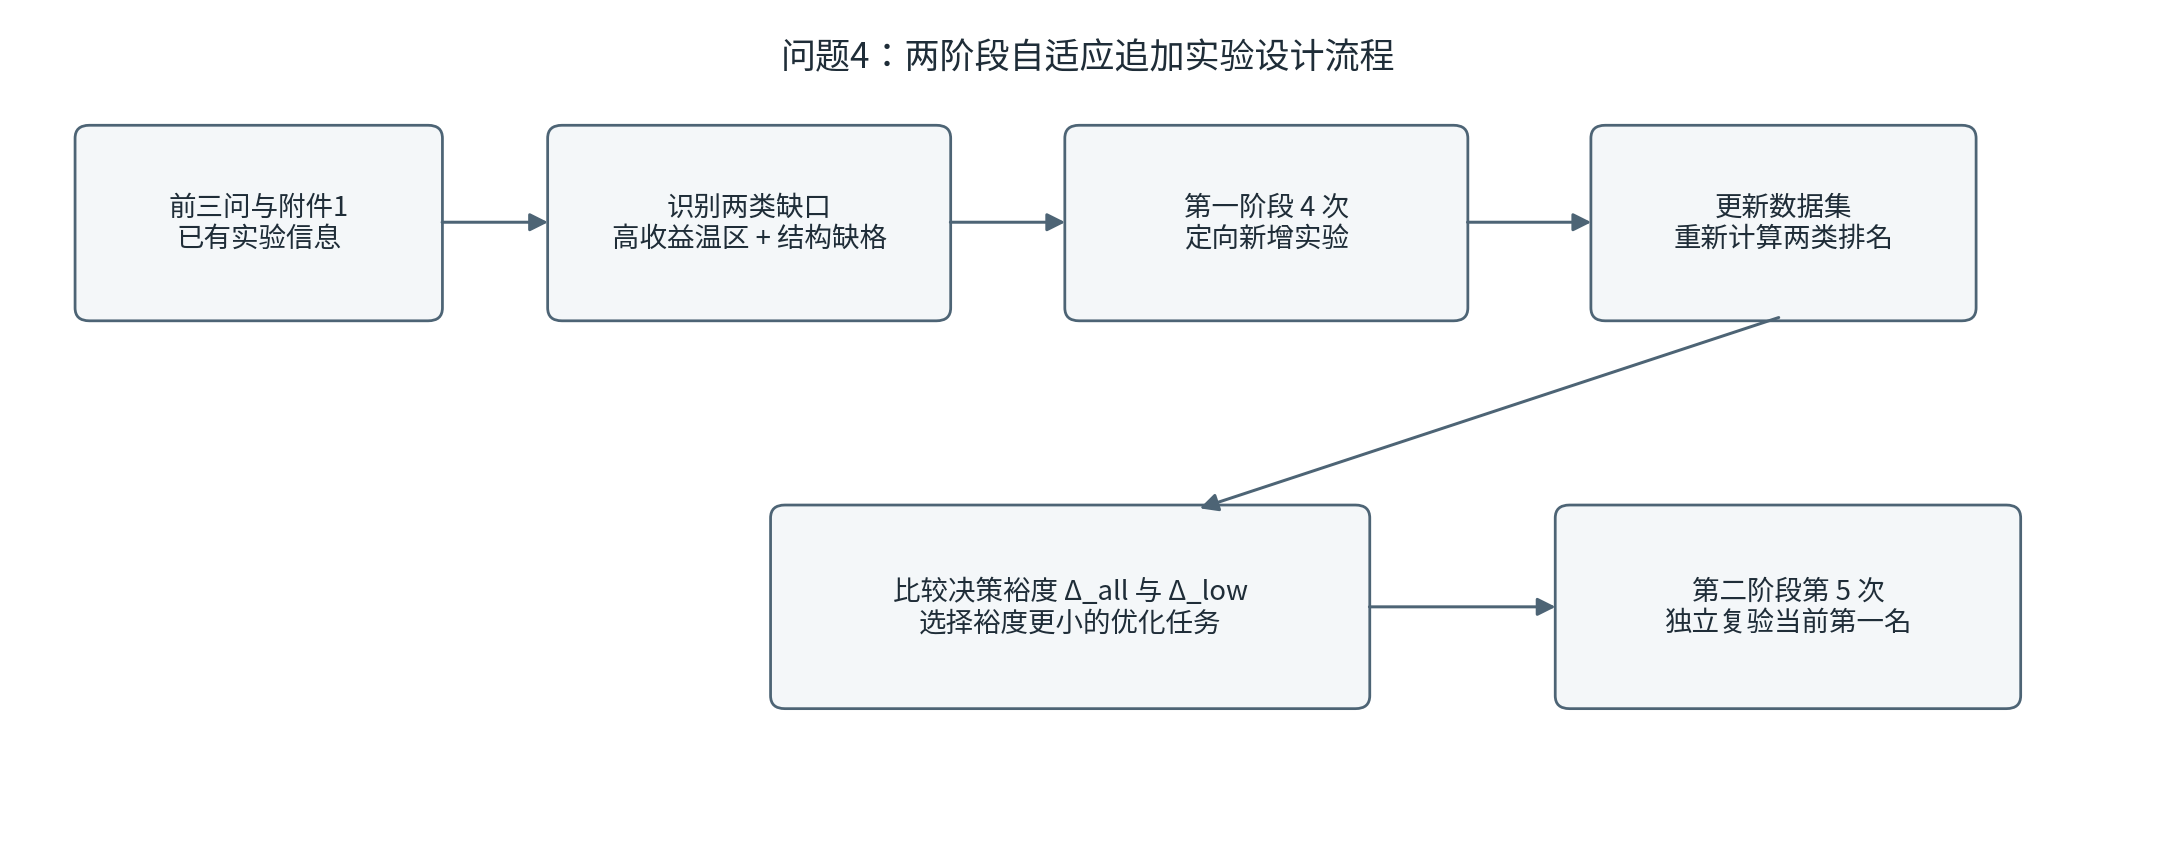
\includegraphics[width=\textwidth]{figures/q4_two_stage_experiment_design.png}
  \caption{两阶段自适应追加实验设计流程}
  \label{fig:q4-flow}
\end{figure}

对每条实测记录，仍沿用百分数尺度下的 $\mathrm{C}_4$ 烯烃收率
\begin{equation}
  Y_{\mathrm{C4}}=\frac{X_{\mathrm{EtOH}}S_{\mathrm{C4}}}{100}.
  \label{eq:q4-yield}
\end{equation}
为保持与已有结果的数值口径一致，式~\eqref{eq:q4-yield} 中的 $X_{\mathrm{EtOH}}$ 按附件表格显示精度取值。由现有观测的两类排名得到表~\ref{tab:q4-initial-rankings}：全温区的第一、第二名间隔为 1.607310 个百分点，严格 $T<\SI{350}{\degreeCelsius}$ 时的对应间隔为 6.464836 个百分点。

\begin{table}[H]
  \centering
  \caption{两类优化任务的当前观测排名与决策裕度}
  \label{tab:q4-initial-rankings}
  \small
  \begin{tabularx}{\textwidth}{L{0.17\textwidth}C{0.16\textwidth}C{0.13\textwidth}C{0.16\textwidth}C{0.13\textwidth}C{0.15\textwidth}}
    \toprule
    优化任务 & 第一名 & $Y_{(1)}$/\% & 第二名 & $Y_{(2)}$/\% & 决策裕度/百分点 \\
    \midrule
    全温区 & A3--400 ℃ & 44.720910 & A3--450 ℃ & 43.113600 & 1.607310 \\
    严格 $T<350$ ℃ & A2--325 ℃ & 17.263556 & A3--325 ℃ & 10.798720 & 6.464836 \\
    \bottomrule
  \end{tabularx}
\end{table}


\subsection{第一阶段：高收益温区与结构缺格的定向补充}

对于仅允许增加一个内部温度点的关键区间 $[a,b]$，在不预设局部响应函数形式的条件下，采用极小最大未观测温度间隔准则：
\begin{equation}
  T^{\star}=\arg\min_{a<T<b}\max\{T-a,b-T\}=\frac{a+b}{2}.
  \label{eq:q4-bisect}
\end{equation}
因此，A3 的 \SIrange{400}{450}{\degreeCelsius} 高收益区取 \SI{425}{\degreeCelsius}，A2 的 \SIrange{325}{350}{\degreeCelsius} 关键低温区取 \SI{337.5}{\degreeCelsius}。该准则只说明补点能均衡缩小温度空档，并不把补点解释为反应最优温度。

其余两次实验用于补齐严格匹配结构在 \SI{400}{\degreeCelsius} 的两个缺格。A4、A1、A2、A6 在催化材料总装料量、配比、乙醇进料条件及装料方式一致时，对应 $0.5,1,2,5$ wt\% 的 Co 负载量；其中仅 A1、A2 尚无 \SI{400}{\degreeCelsius} 记录。同时，A1/A3 和 A2/A5 分别构成仅乙醇进料条件不同的严格匹配对，且 A3、A5 已有 \SI{400}{\degreeCelsius} 记录。故 A1--\SI{400}{\degreeCelsius}、A2--\SI{400}{\degreeCelsius} 可同时补充高温 Co 负载量响应和两组进料对照信息。

\begin{table}[H]
  \centering
  \caption{第一阶段四次定向追加实验}
  \label{tab:q4-phase-one}
  \small
  \begin{tabularx}{\textwidth}{C{0.09\textwidth}C{0.18\textwidth}C{0.13\textwidth}X}
    \toprule
    实验 & 条件 & 温度 & 类型与作用 \\
    \midrule
    E1 & A3 原条件 & 425 ℃ & 组内单点二分加密，细化 400--450 ℃高收益区 \\
    E2 & A2 原条件 & 337.5 ℃ & 组内单点二分加密，细化严格低温区 325--350 ℃ \\
    E3 & A2 原条件 & 400 ℃ & 受控高温扩展；补 2 wt\% Co 高温缺格及 A2/A5 进料对照 \\
    E4 & A1 原条件 & 400 ℃ & 受控高温扩展；补 1 wt\% Co 高温缺格及 A1/A3 进料对照 \\
    \bottomrule
  \end{tabularx}
\end{table}


图~\ref{fig:q4-a3-design} 和图~\ref{fig:q4-a2-design} 分别以虚线标出两个组内补点；虚线不对应任何预设收率。图~\ref{fig:q4-co-profile} 和表~\ref{tab:q4-co-profile} 显示 \SI{400}{\degreeCelsius} 横截面中 A1、A2 的现有缺格，表~\ref{tab:q4-feed-pairs} 进一步列出两组乙醇进料严格匹配对的补全位置。

\begin{figure}[H]
  \centering
  \begin{subfigure}[b]{0.49\textwidth}
    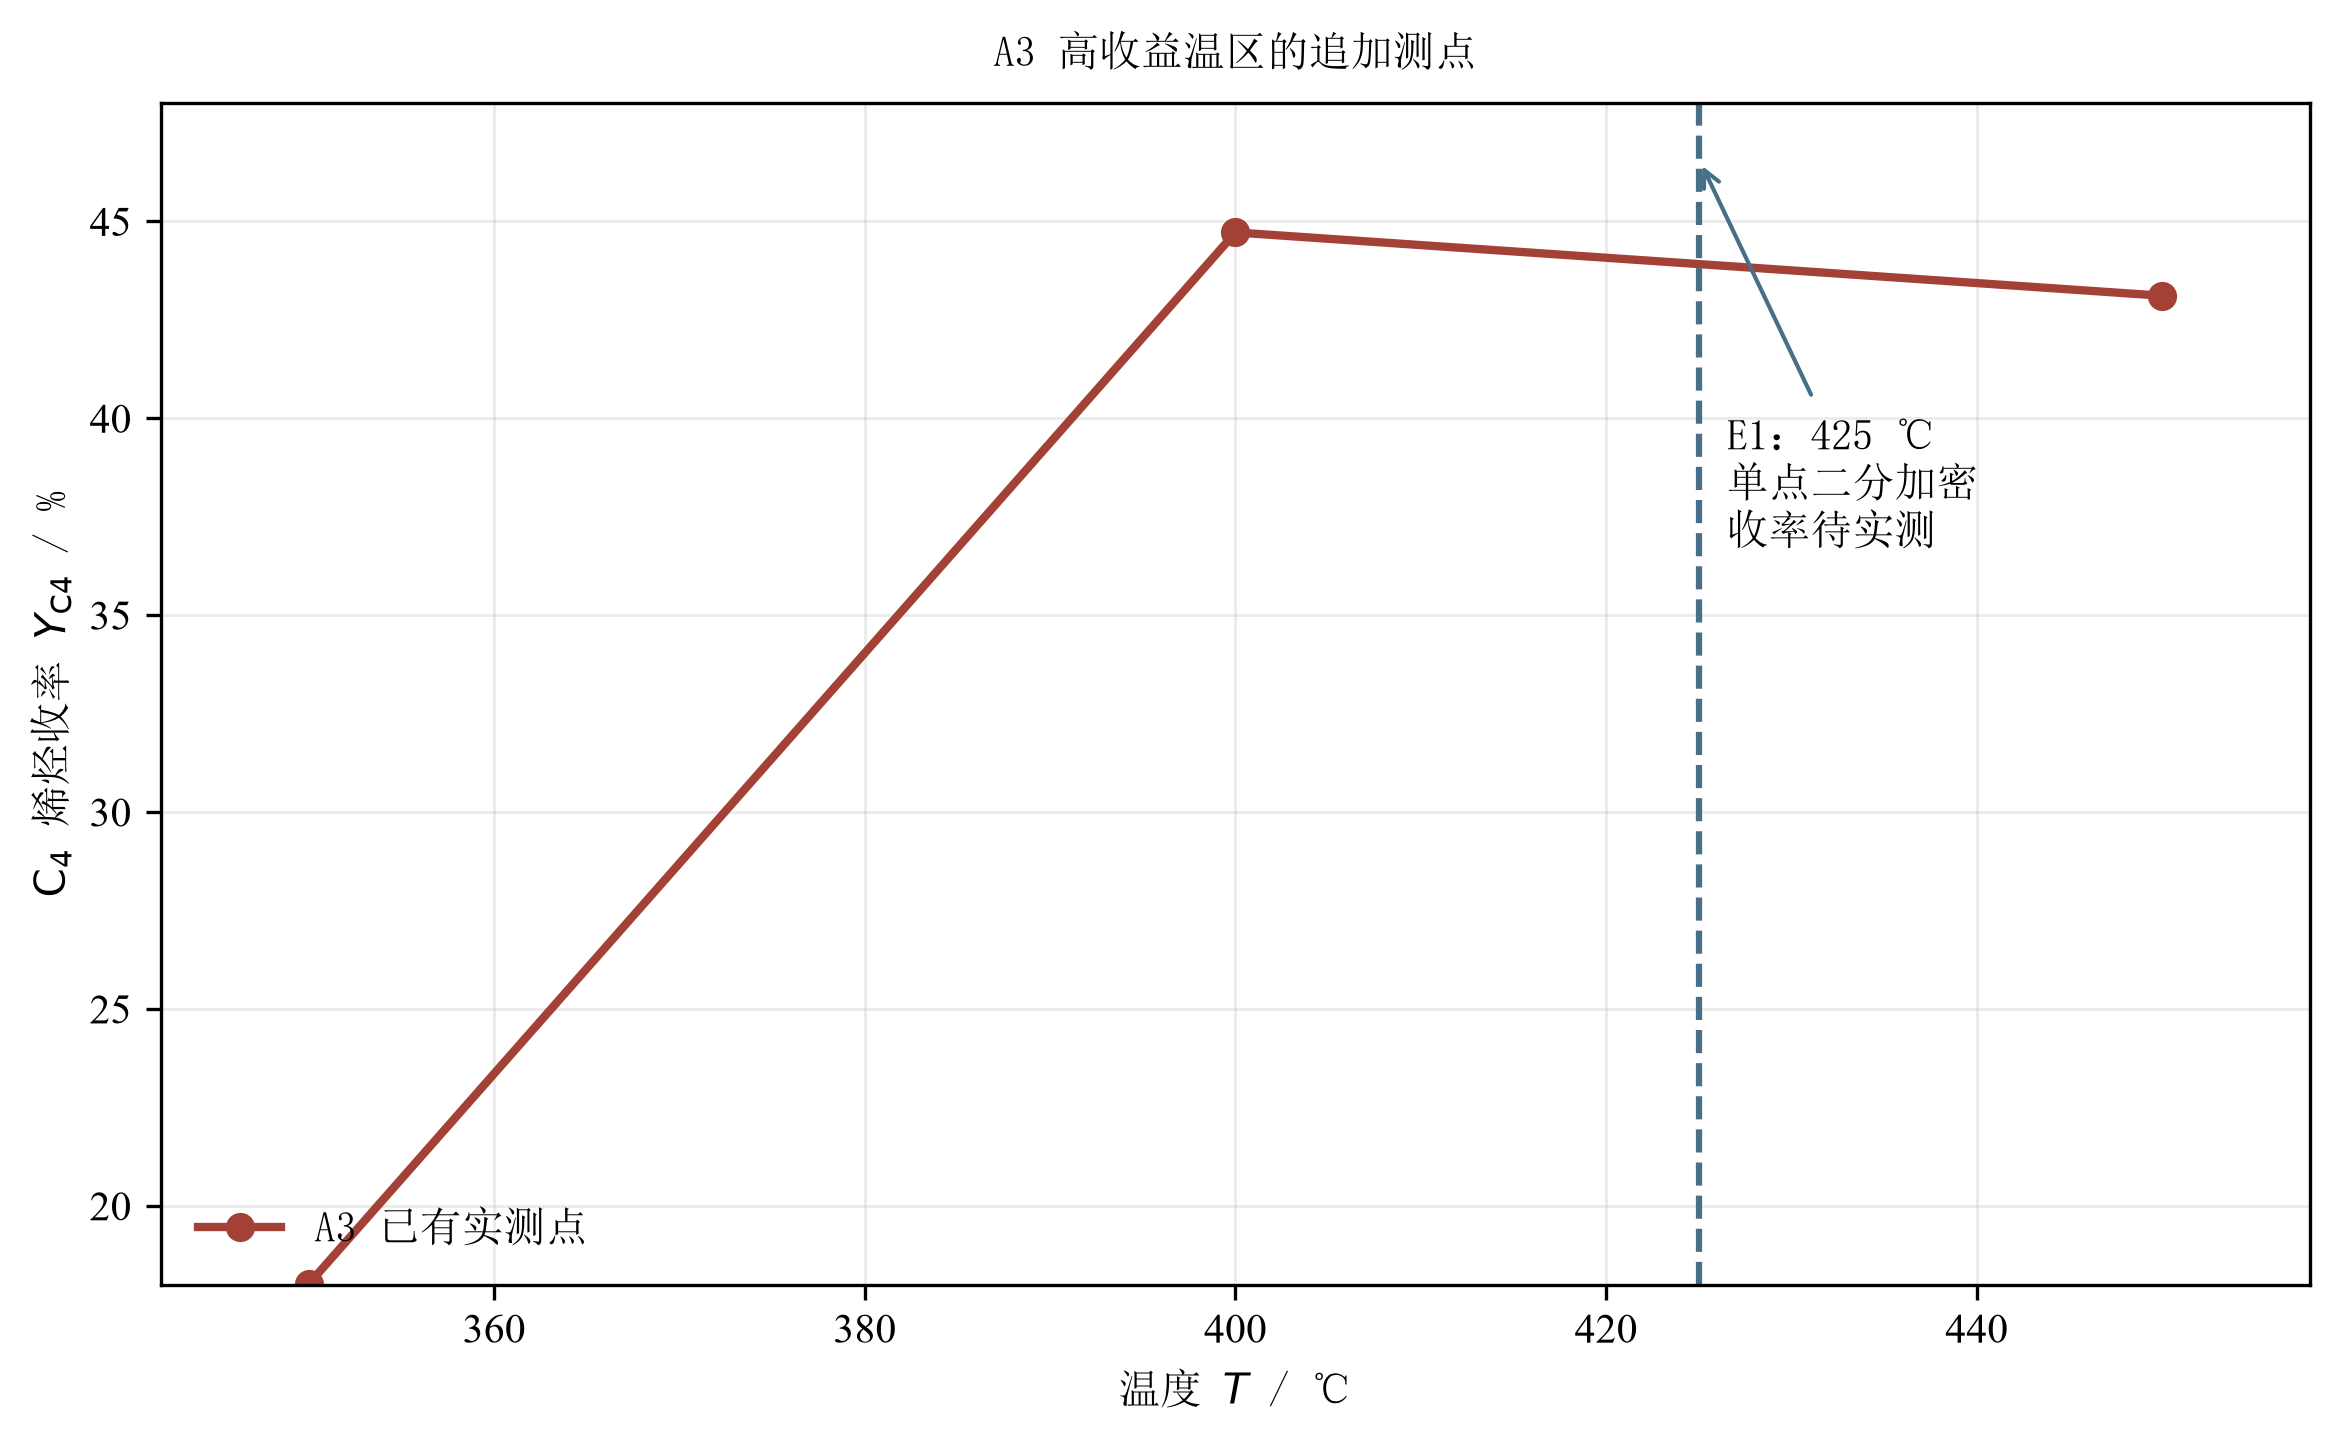
\includegraphics[width=\textwidth]{figures/q4_a3_high_temperature_design.png}
    \caption{A3 高收益温区}
    \label{fig:q4-a3-design}
  \end{subfigure}
  \begin{subfigure}[b]{0.49\textwidth}
    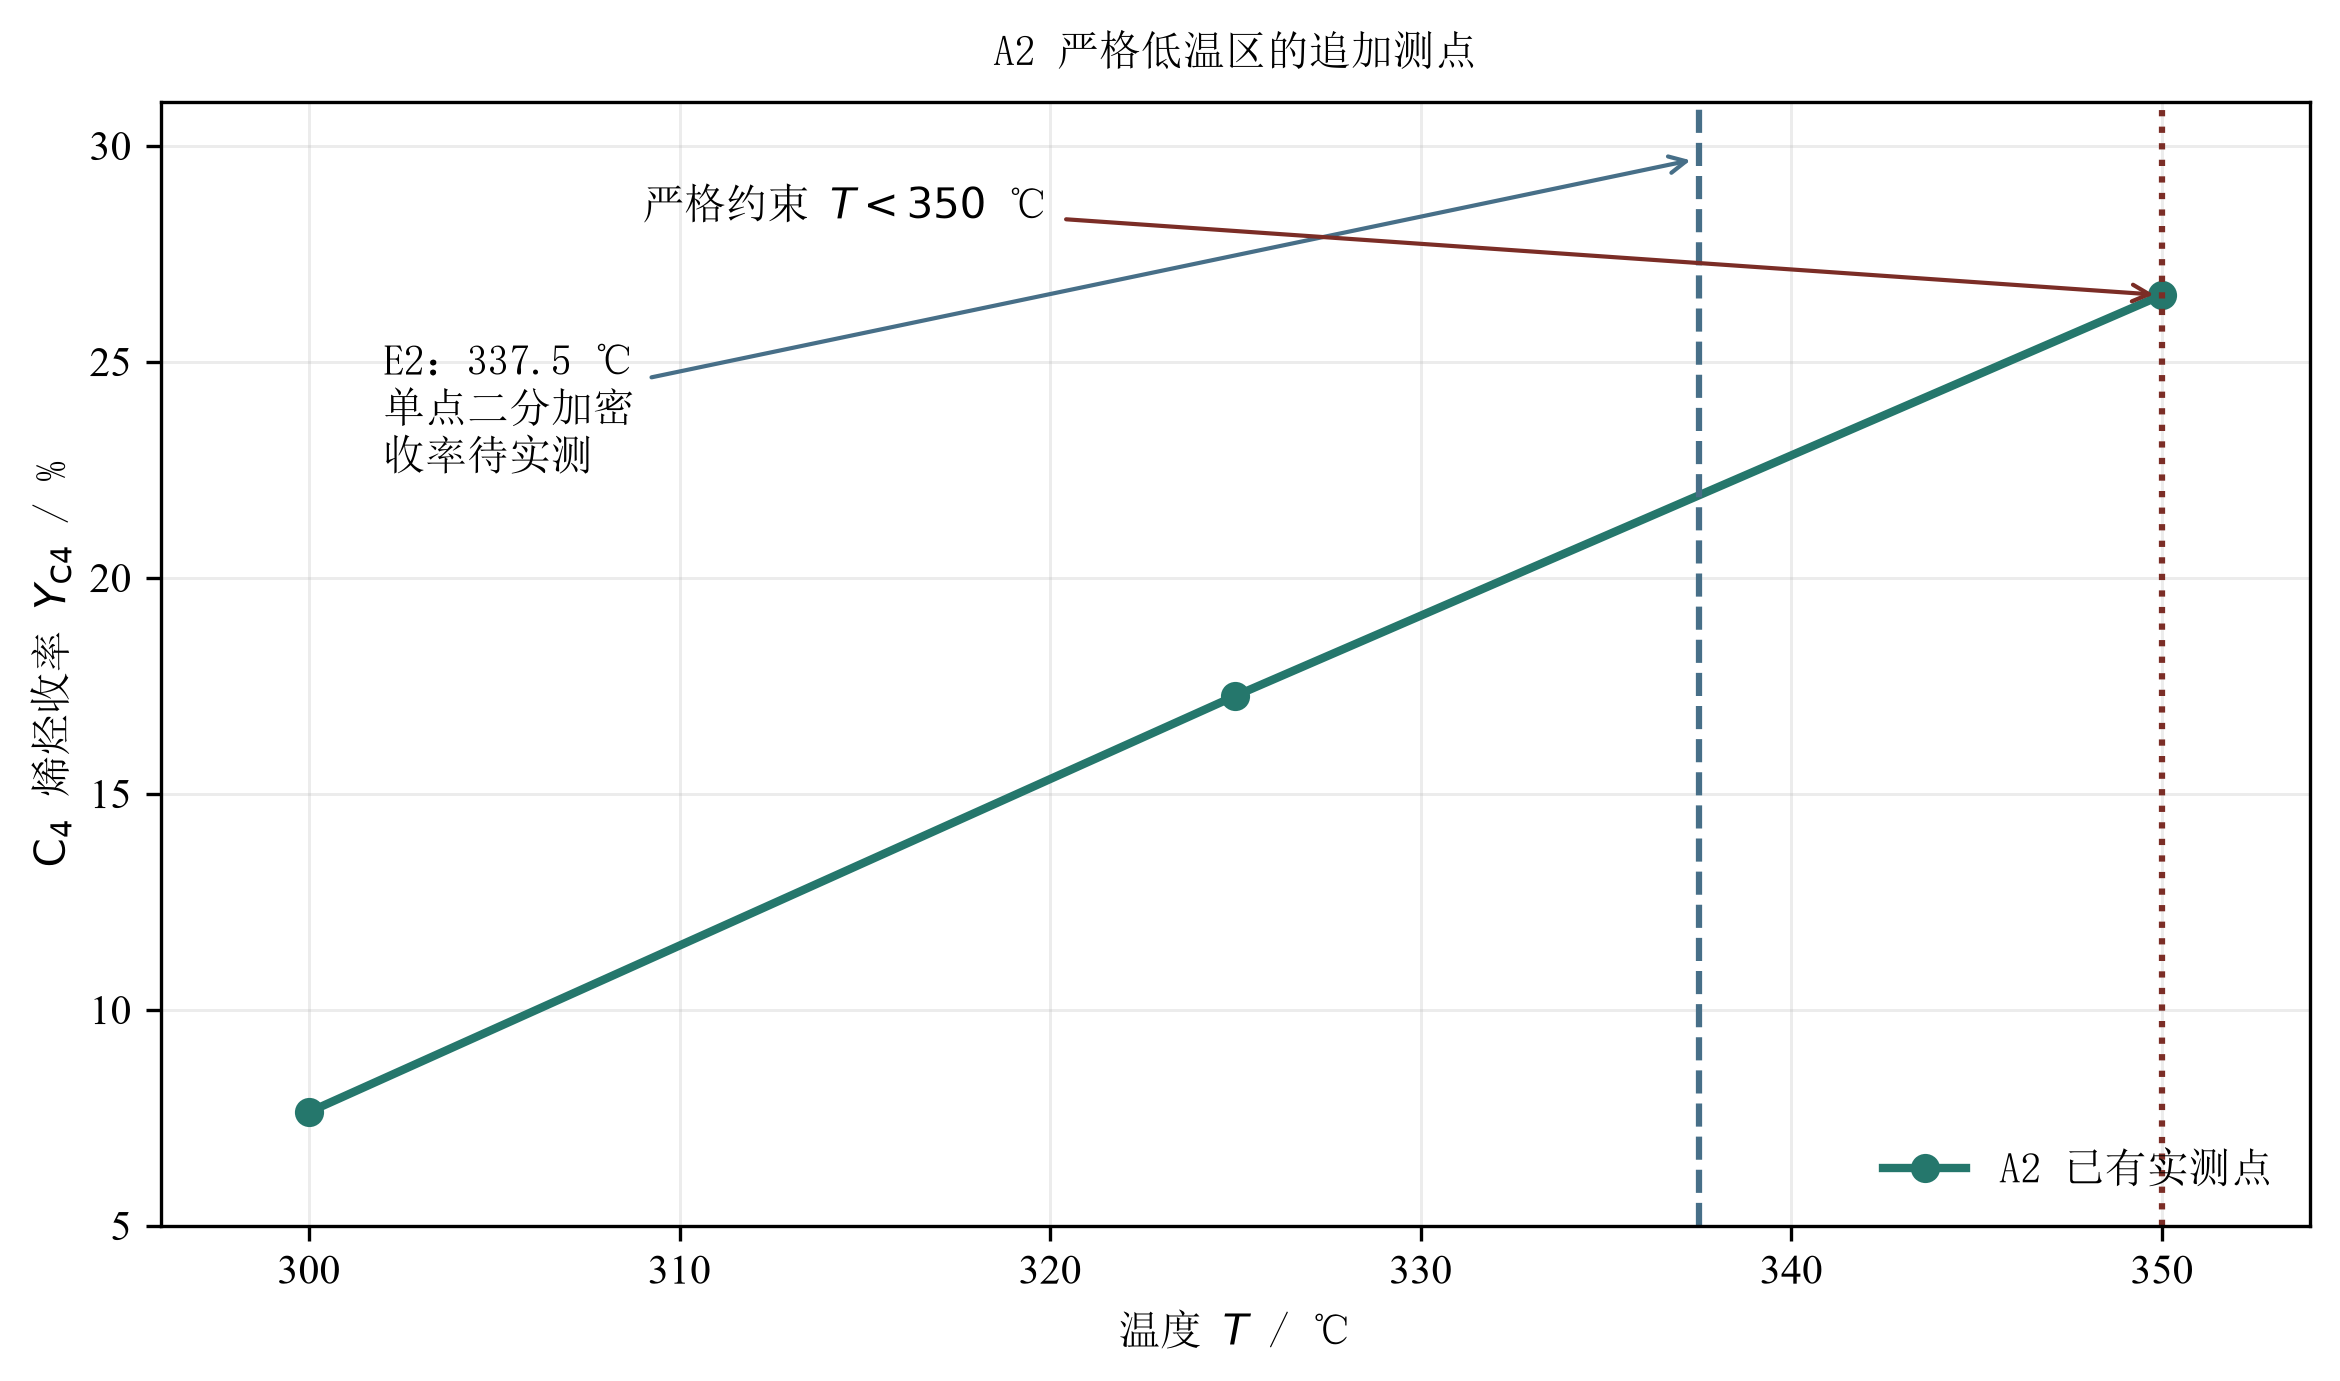
\includegraphics[width=\textwidth]{figures/q4_a2_low_temperature_design.png}
    \caption{A2 严格低温区}
    \label{fig:q4-a2-design}
  \end{subfigure}
  \caption{第一阶段的两个组内温度加密点}
\end{figure}

\begin{figure}[H]
  \centering
  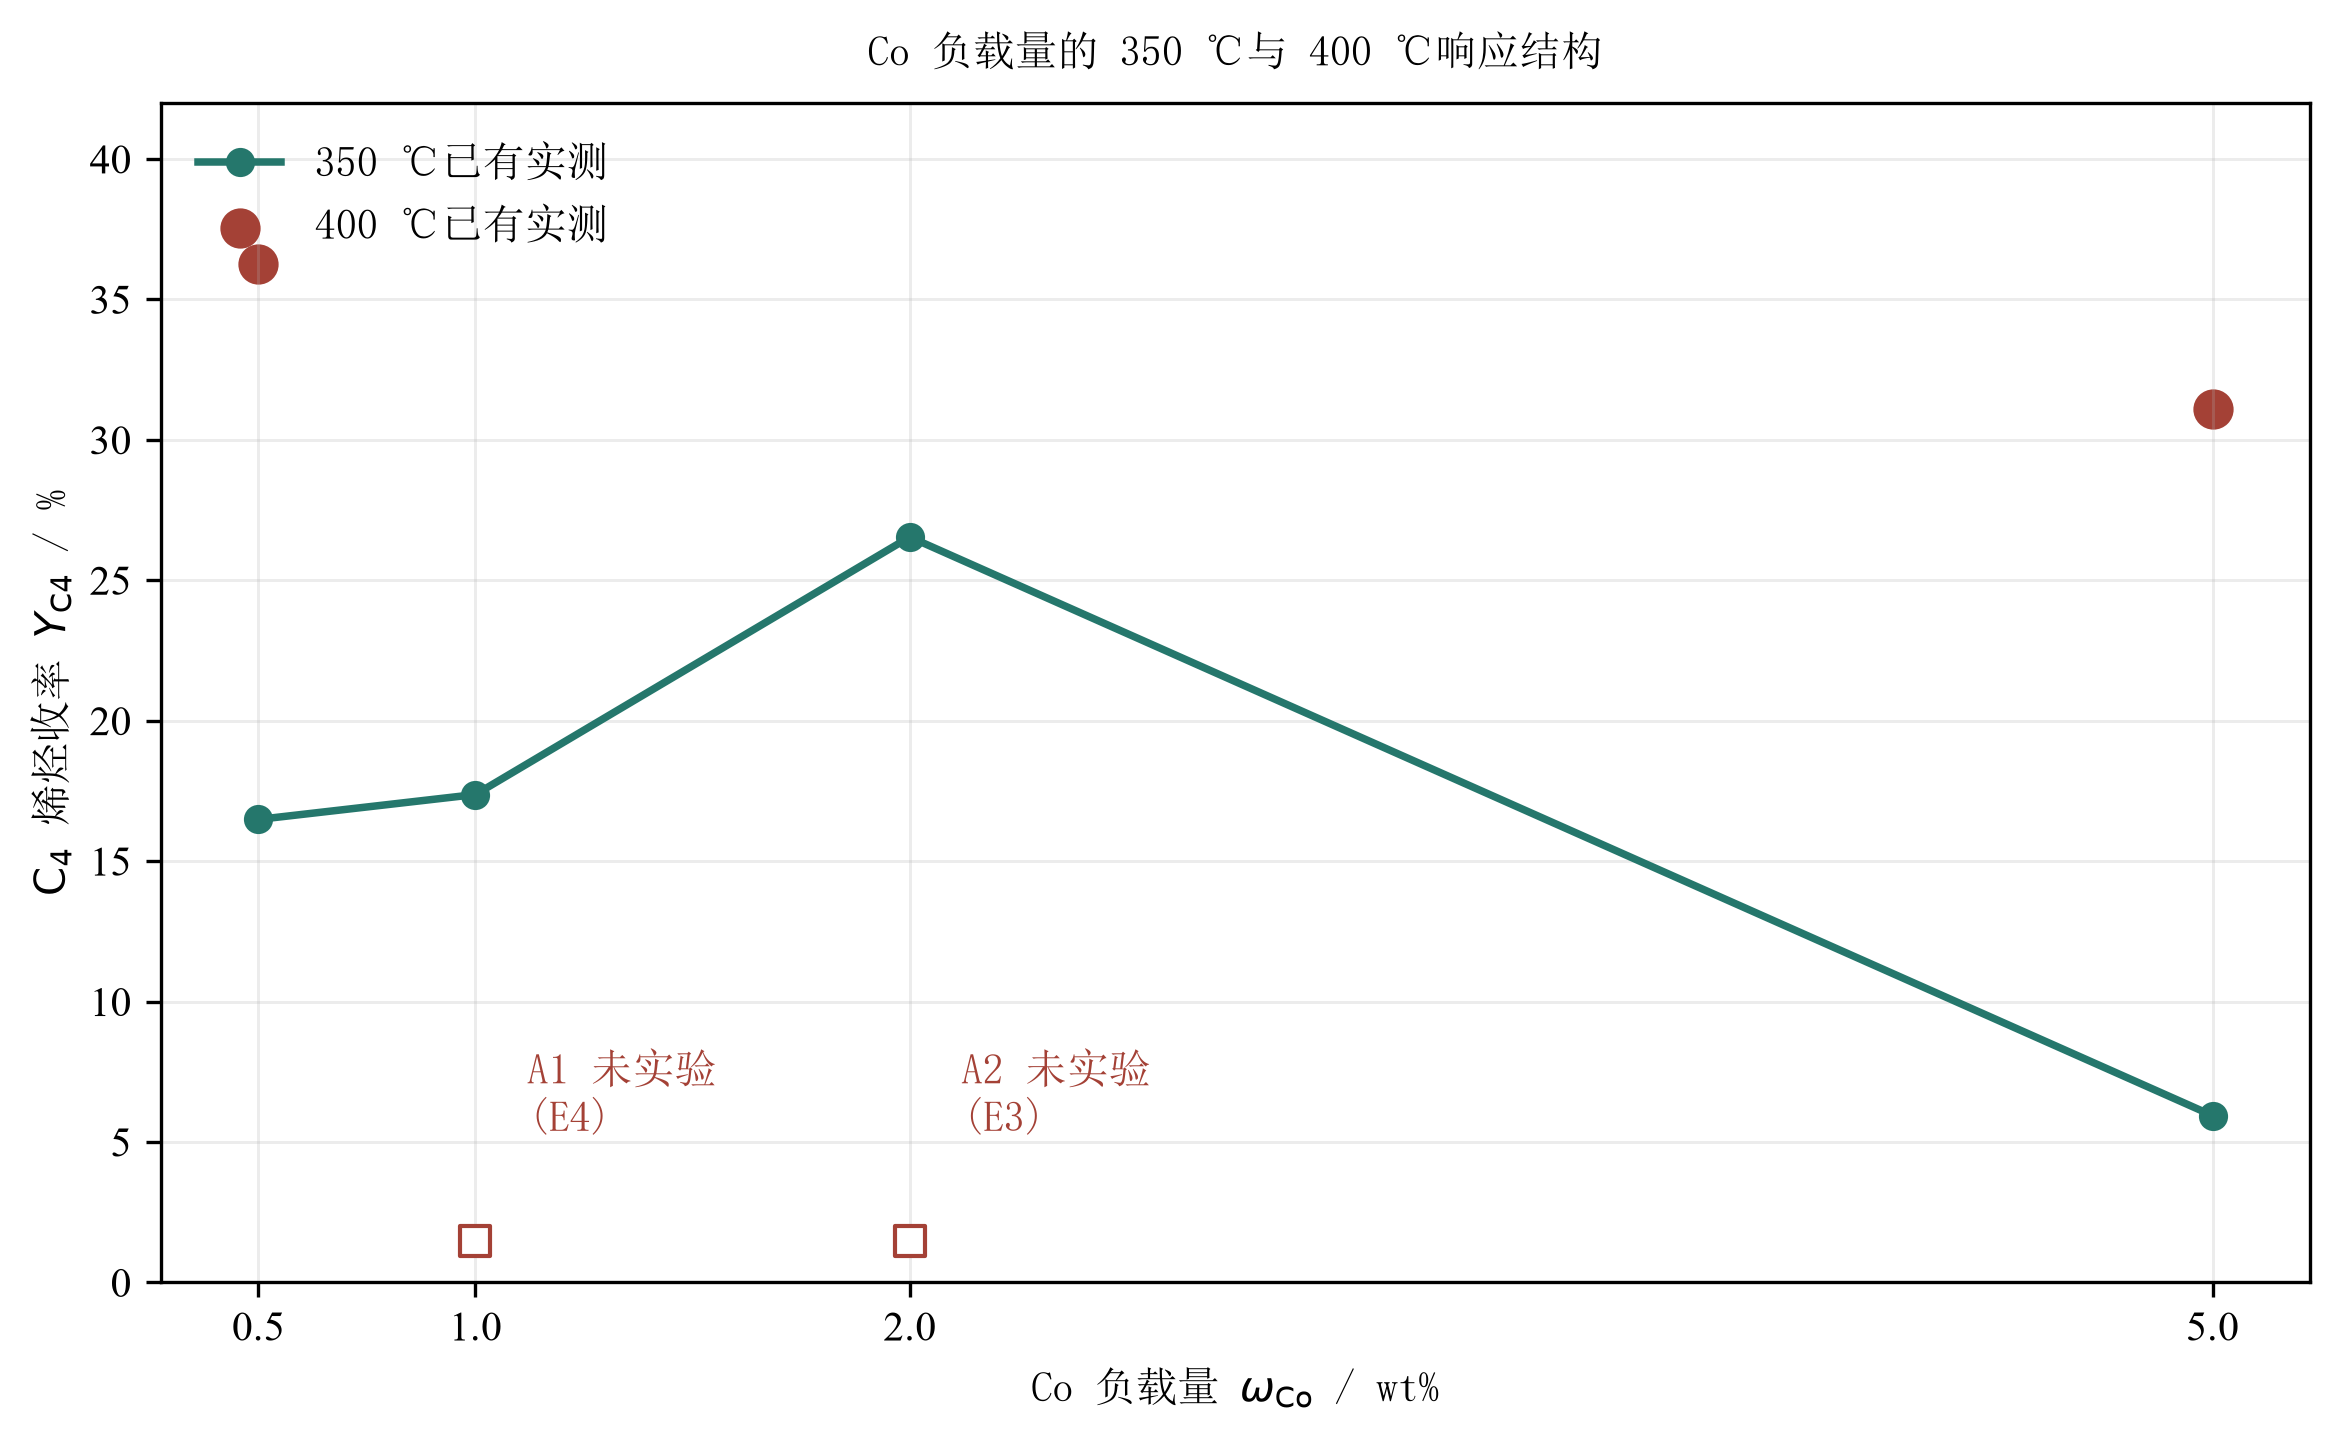
\includegraphics[width=0.84\textwidth]{figures/q4_co_loading_profile_design.png}
  \caption{Co 负载量严格匹配块在 \SI{350}{\degreeCelsius} 与 \SI{400}{\degreeCelsius} 的现有响应结构；下方空心方块表示待补的实测位置，不表示收率数值}
  \label{fig:q4-co-profile}
\end{figure}

\begin{table}[H]
  \centering
  \caption{Co 负载量严格匹配块的现有收率结构}
  \label{tab:q4-co-profile}
  \small
  \begin{tabularx}{\textwidth}{C{0.14\textwidth}C{0.18\textwidth}C{0.18\textwidth}C{0.18\textwidth}C{0.18\textwidth}}
    \toprule
    温度 & 0.5 wt\% (A4) & 1 wt\% (A1) & 2 wt\% (A2) & 5 wt\% (A6) \\
    \midrule
    350 ℃ & 16.48625 & 17.37328 & 26.54108 & 5.94270 \\
    400 ℃ & 36.26168 & 未实验 & 未实验 & 31.09589 \\
    \bottomrule
  \end{tabularx}
\end{table}

\begin{table}[H]
  \centering
  \caption{400 ℃乙醇进料严格匹配对的补全安排}
  \label{tab:q4-feed-pairs}
  \small
  \begin{tabularx}{\textwidth}{C{0.15\textwidth}C{0.17\textwidth}C{0.18\textwidth}C{0.18\textwidth}C{0.18\textwidth}}
    \toprule
    严格匹配对 & 仅改变因素 & 前者 400 ℃收率/\% & 后者 400 ℃收率/\% & 补全安排 \\
    \midrule
    A1/A3 & 乙醇进料条件 & 未实验 & 44.72091 & E4：A1--400 ℃ \\
    A2/A5 & 乙醇进料条件 & 未实验 & 29.05480 & E3：A2--400 ℃ \\
    \bottomrule
  \end{tabularx}
\end{table}


综上，第一阶段实验集合为
\begin{equation}
  \mathcal{E}_{1}=\{(\mathrm{A3},425),(\mathrm{A2},337.5),(\mathrm{A2},400),(\mathrm{A1},400)\},
  \qquad
  \mathcal{D}_{4}=\mathcal{D}_{0}\cup\mathcal{E}_{1}.
  \label{eq:q4-phase-one}
\end{equation}
其中 A3--\SI{425}{\degreeCelsius} 与 A2--\SI{337.5}{\degreeCelsius} 均位于各自已有温度范围内；A1/A2--\SI{400}{\degreeCelsius} 则属于有严格匹配结构支撑的受控高温扩展，实施前需确认设备、安全与材料可行性。若设备温控分辨率不能精确设定 \SI{337.5}{\degreeCelsius} 或 \SI{425}{\degreeCelsius}，应取最近可实现设定值，且前者仍须严格小于 \SI{350}{\degreeCelsius}。

\subsection{第二阶段：决策裕度导向的独立复验}

完成第一阶段后，分别在全温区和严格低温区内按实测收率重新确定第一、第二名，记为 $Y^{s}_{(1)}$、$Y^{s}_{(2)}$，其中 $s\in\{\mathrm{all},\mathrm{low}\}$。定义观测排名的决策裕度为
\begin{equation}
  \Delta_s=Y^{s}_{(1)}-Y^{s}_{(2)},
  \qquad
  s^{\star}=\arg\min_{s\in\{\mathrm{all},\mathrm{low}\}}\Delta_s.
  \label{eq:q4-margin}
\end{equation}
第 5 次实验 E5 对任务 $s^{\star}$ 的当前第一名进行一次新的独立实验运行。复验应保持催化剂组成、装料量、装料方式、乙醇进料条件、温度、测量时刻及操作检测规程与被复验条件一致。

在不同候选条件的实验波动量级大致可比较这一弱前提下，较小的 $\Delta_s$ 表示前两名的观测间隔更小，因而优先安排复验。该量仅作为实验排序的决策裕度，不作为显著性、置信区间或方差估计。若两类决策裕度在保留精度下相同，则应如实报告并列，结合实验安全性与实际工艺优先级确定复验对象。

若原始观测收率为 $Y_1$、独立复验收率为 $Y_2$，可报告重复均值和两次观测的样本方差：
\begin{equation}
  \overline{Y}=\frac{Y_1+Y_2}{2},
  \qquad
  s_r^2=\frac{(Y_1-Y_2)^2}{2}.
  \label{eq:q4-repeat-summary}
\end{equation}
由于仅有两次观测，上述统计量只提供基本的重复性描述；新增实验结果获得后，再据实更新两类任务的排名、E5 的复验对象及式~\eqref{eq:q4-repeat-summary} 的汇总值。

\subsection{设计边界}

本方案的 5 次预算集中用于两个高价值温度空档、两个具有严格匹配支撑的结构缺格和一次独立复验，未将同一组合的多温度记录视为大量同质独立催化剂设计，也未将 A11 作为普通 $\rho$ 配比点。由于每个新增条件初始仍只有一次观测，补齐 \SI{400}{\degreeCelsius} 横截面后只能形成完整响应剖面，不能据此进行有纯误差支持的完整双因素方差分析；一次独立复验也不足以建立可靠的总体实验误差分布。

\section{模型评价与改进}

本文的评价对象是由数据结构、模型边界和求解规则共同构成的整体框架，而非孤立评价某一算法。针对稀疏、非正交且缺少重复测量的实验数据，框架优先保证结论可追溯，再在相应边界内追求信息利用效率。

\subsection{模型优点}

\begin{enumerate}
  \item \textbf{本模型将数据层级与问题目标一一对应。} 问题一只在同一催化剂组合内刻画温度响应，问题二才在严格匹配背景下比较因素，问题三再把转化率和选择性合成为收率优化目标。由此避免将 114 条温度记录误作 114 个独立催化剂设计，也避免以单项响应替代收率判断。
  \item \textbf{本模型以低复杂度规则约束小样本拟合。} 问题一的一次--二次候选、组内留一预测和物理边界检查相互制衡；问题三用分段线性连续化保持相邻节点连续而不制造内部峰值。该设计把“拟合得更好”与“可用于排序”明确区分，符合小样本交叉验证应审慎解释的原则\cite{stone1974,arlot2010,hastie2009}。
  \item \textbf{本模型保留了条件效应的证据路径。} 每一因素结论都可追溯至具体的匹配背景、共同温度与离散水平；同一因素在不同背景中反转时，模型报告反转而不强行汇总为一个全局主效应。局部二阶对比只在四格齐全时计算，并以删一温度检验符号是否由单点驱动。
  \item \textbf{本模型把优化与后续实验衔接起来。} 问题四将新增预算分配给高收益温区的空档、严格匹配结构的缺格和独立复验，既服务于当前推荐，也服务于下一轮可比较证据的形成；这与实验设计中以对照结构和重复性支撑解释的思想一致\cite{montgomery2017,box2005}。
\end{enumerate}

\subsection{模型不足}

\begin{enumerate}
  \item \textbf{本模型的优化域受实验覆盖限制。} 分段线性规则只在同一组合的相邻实测温度之间有效，候选因素级代理在留出高收益组合时误差较大。因此，未实验配方、跨组合连续设计空间和区间外温度均不能据此宣称最优。
  \item \textbf{本模型不能从无重复条件中分离纯实验误差。} 附件1大部分“组合--温度”单元只有一次观测；留一误差、删一温度敏感性和两次复验的样本方差分别刻画预测稳定性、单点驱动风险和基础重复性，均不等同于完整的显著性检验或总体方差估计。
  \item \textbf{本模型对可比较结构具有依赖性。} 严格匹配会主动舍弃无法控制其余因素的记录，以换取解释清晰度；当后续新增实验进入新的因素区域时，原有匹配块和局部四格未必仍存在，需要按新的实际设计重新枚举。
  \item \textbf{本模型不赋予机理因果解释。} 催化材料性质与反应路径在文献中具有复杂耦合\cite{pomalaza2016,hanspal2017,cimino2018}，而本文数据未包含表征、动力学或重复实验信息，故不能把条件差异解释为特定活性位或反应步骤的因果贡献。
\end{enumerate}

\subsection{模型改进方向}

\begin{enumerate}
  \item 在问题二已出现方向反转的匹配背景，以及问题三高收益候选附近，优先增加同条件重复实验；获得纯误差后，可将当前的条件差分扩展为带不确定性的区间比较。
  \item 在保持温度层和关键因素平衡的前提下补充正交或近正交设计点，再建立受层级约束的响应面或层次模型；模型拟合、交叉验证和优化应使用彼此隔离的验证单元。
  \item 对问题四第一阶段的新增实测结果，先更新观测排序、严格匹配块和决策裕度，再按预定规则确定复验对象；若出现新的高收益区域，应以实际新增点为起点重新设计后续温度加密，而不是沿用旧曲线的外推峰值。
\end{enumerate}

\section{结论}

\subsection{问题一：温度响应与时间变化}

在附件1的 21 个催化剂组合中，乙醇转化率从各自最低实测温度到最高实测温度均总体提高，其中 19 组逐点增加；$\mathrm{C}_4$ 烯烃选择性则表现出明显的组合差异，15 组逐点增加，其余组合出现局部回落或平台。以组内留一预测、原始散点和 0--100\% 边界共同筛选后，乙醇转化率有 15 组采用二次经验描述、5 组采用线性总体描述，A11 不强行确定具体低阶函数；选择性有 12 组采用二次描述、8 组采用线性总体描述，A6 仅作粗略描述。

附件2中，乙醇转化率由 43.5474\%（20 min）降至 29.9060\%（273 min），观测窗内的线性平均变化为 $X_{\mathrm{EtOH}}(t)=42.6709-0.05276t$，$R^2=0.9329$、$\mathrm{RMSE}_{\mathrm{LOO}}=2.025$ 个百分点。7 个离散时刻的 $\mathrm{C}_4$ 烯烃收率均依次下降；选择性在 36.72\%--40.32\% 间波动。因此，结论仅描述当前时间窗的变化，不将其外推为长期稳定性或催化剂失活机理。

\subsection{问题二：催化因素与温度的条件影响}

在 250--350 ℃的共同温区，21 个组合的乙醇转化率和 $\mathrm{C}_4$ 烯烃选择性端点差均为正，平均分别为 24.46 和 15.30 个百分点，温度端点促进方向在已有组合中最一致。严格匹配和跨背景对比同时显示，催化因素并不存在脱离背景的统一优劣：Co 负载量由 1 wt\% 增至 5 wt\% 时，转化率在两个匹配背景中分别出现 $+11.93$ 和 $-2.78$ 个百分点的平均差，而选择性在两个背景中的平均差均为负；乙醇进料条件和装料方式也均呈背景依赖。

在当前五因素定义下，仅 $(m_{\mathrm{cat}},q_{\mathrm{EtOH}})$ 与 $(q_{\mathrm{EtOH}},z)$ 形成完整局部四格。后者在 \SI{350}{\degreeCelsius} 的二阶对比为 $I_{X_{\mathrm{EtOH}}}=3.07$、$I_{S_{\mathrm{C4}}}=-19.41$ 个百分点，且两套四格删去任一共同温度后的平均二阶对比均保持原符号。上述结果描述的是离散水平、实际共同温度和指定背景下的局部非加性，不延伸为全局交互强度或严格因果判断。

\subsection{问题三：实验支持域内的收率优化}

以 $Y_{\mathrm{C4}}=X_{\mathrm{EtOH}}S_{\mathrm{C4}}/100$ 衡量联合条件的实测表现。无温度限制时，A3--\SI{400}{\degreeCelsius} 的实测 $\mathrm{C}_4$ 烯烃收率最高，为 44.72\%，对应 $X_{\mathrm{EtOH}}=83.70\%$、$S_{\mathrm{C4}}=53.43\%$；在各组合自身实测温区内的分段线性连续化下，该结论不产生新的内部峰值。

严格 $T<\SI{350}{\degreeCelsius}$ 时，实测最优为 A2--\SI{325}{\degreeCelsius}，收率 17.26\%。利用 A2 的 325--350 ℃相邻点构造的局部线性函数在 $T\to350^{-}$ 时给出 26.54\% 的上确界，但 \SI{350}{\degreeCelsius} 不属于严格可行域，故该数值不是可直接取得的最大收率。候选因素级代理在留出 A3 组时对其 44.72\% 的实际收率仅给出 17.99\%--26.80\% 的预测，因此不对未实验配方进行最优排序。

\subsection{问题四：5 次新增实验的安排}

第一阶段安排 4 次定向实验：A3--\SI{425}{\degreeCelsius} 和 A2--\SI{337.5}{\degreeCelsius} 用于分别细化高收益温区和严格低温区；A1--\SI{400}{\degreeCelsius} 与 A2--\SI{400}{\degreeCelsius} 用于补齐 Co 负载量和乙醇进料严格匹配中的关键缺格。完成后，按新增实测收率重新计算全温区与严格低温区的第一、第二名间隔；第 5 次独立复验间隔较小任务的当前第一名，并报告两次观测的均值和样本方差。该方案提供的是可执行的实验顺序，新增点的实际收率及最终复验对象须待实测后据实确定。

\begin{thebibliography}{99}
  \bibitem{pomalaza2016} Pomalaza G, Capron M, Ordomsky V, et al. Recent breakthroughs in the conversion of ethanol to butadiene[J]. Catalysts, 2016, 6(12): 203.
  \bibitem{hanspal2017} Hanspal S, Young Z D, Prillaman J T, et al. Influence of surface acid and base sites on the Guerbet coupling of ethanol to butanol over metal phosphate catalysts[J]. Journal of Catalysis, 2017, 352: 182--190.
  \bibitem{lovon2017} Lov\'on-Quintana J J, Rodriguez-Guerrero J K, Valen\c{c}a P G. Carbonate hydroxyapatite as a catalyst for ethanol conversion to hydrocarbon fuels[J]. Applied Catalysis A: General, 2017, 542: 136--145.
  \bibitem{cimino2018} Cimino S, Lisi L, Romanucci S. Catalysts for conversion of ethanol to butanol: Effect of acid-base and redox properties[J]. Catalysis Today, 2018, 304: 58--63.
  \bibitem{fihri2017} Fihri A, Len C, Varma R S, et al. Hydroxyapatite: A review of syntheses, structure and applications in heterogeneous catalysis[J]. Coordination Chemistry Reviews, 2017, 347: 48--76.
  \bibitem{stone1974} Stone M. Cross-validatory choice and assessment of statistical predictions[J]. Journal of the Royal Statistical Society: Series B (Methodological), 1974, 36(2): 111--133.
  \bibitem{arlot2010} Arlot S, Celisse A. A survey of cross-validation procedures for model selection[J]. Statistics Surveys, 2010, 4: 40--79.
  \bibitem{montgomery2017} Montgomery D C. Design and analysis of experiments[M]. 9th ed. Hoboken: John Wiley \& Sons, 2017.
  \bibitem{box2005} Box G E P, Hunter J S, Hunter W G. Statistics for experimenters: Design, innovation, and discovery[M]. 2nd ed. Hoboken: John Wiley \& Sons, 2005.
  \bibitem{hastie2009} Hastie T, Tibshirani R, Friedman J. The elements of statistical learning: Data mining, inference, and prediction[M]. 2nd ed. New York: Springer, 2009.
\end{thebibliography}


\appendix
\clearpage
\section*{附录}
\addcontentsline{toc}{section}{附录}
\input{sections/13_appendix}

\end{document}
